In this chapter I describe the process of designing and implementing the PoC solution.

\section{PoC implementation}

I started by implementing a simple Android application that acts as a server for incoming Bluetooth connections from paired devices.
This was fairly straightforward since Android's documentation is up to date and there is a large community of developers for this OS.

The next step was to choose and integrate a smartwatch.

Initially I meant to use the Xiaomi Mi Band 4 since I already owned one.
However, Xiaomi watches do not pair directly with the phone, but with a proprietary application using server-based pairing,
and there is no way to access the data from the phone other than to reverse engineer the protocol, root the phone, and access the pairing keys in the app's database~\cite{miband4-server-based}.

I looked at multiple vendors' popularity based on market share and affordability, their documentation to see how good their development support is and whether or not they have public APIs for development.

According to Statista.com~\ref{fig:watch_market_share}, the most popular are Apple watches, followed by Samsung, Fitbit and other vendors.

\begin{figure}[h]
    \tmpframe{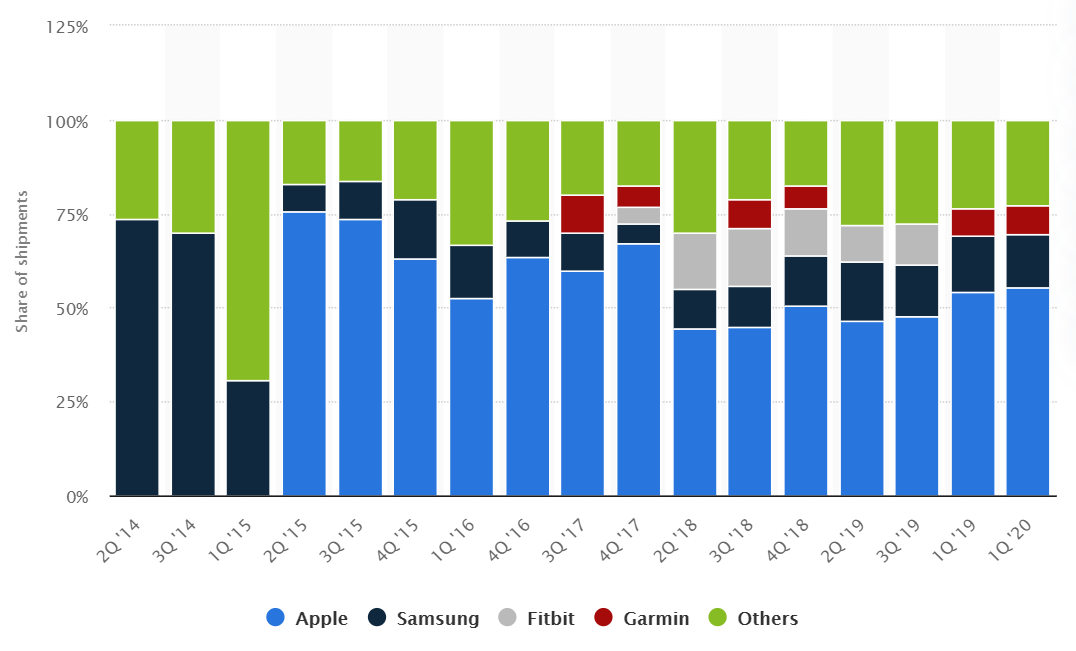
\includegraphics[width=\textwidth]{smartwatch_market_share.png}}
    \caption{Market share of smartwatch unit shipments worldwide from summer 2014 to spring 2020, by vendor~\cite{watch_market_share}.}
    \label{fig:watch_market_share}
\end{figure}

While Apple has a crushing lead on all other vendors, buying a unit just for development is not an option for me because of their high prices.
This is why I chose the Samsung Galaxy Watch Active.

Samsung watches run Tizen OS, which has public APIs, extensive documentation, tutorials and a large community.
This is why I was surprised to find out how difficult it is to develop for this watch.
The watch needs to be connected over the local network to the Tizen Studio IDE;
the tutorial for this~\cite{tizen_connect_tutorial} omits the important step of enabling developer options when working with Bluetooth,
so that the device does not disconnect when trying to use the Bluetooth API.
The tutorial also doesn't mention that Bluetooth should not only be disabled, but has to be turned off, on, and off again in order to connect.

Working with Bluetooth itself was tricky as well since their guide~\cite{tizen_bluetooth_guide} explicitly says that it should be implemented in the main thread,
but the app refused to connect to the phone when it was implemented that way.
When I finally found a working sample application~\cite{tizen_bluetooth_sample}, its Bluetooth functionality was divided into different threads.

When implementing the watch's communication with the Android phone, another surprise was the missing step of asking for permissions to access the heart rate sensor~\cite{tizen_sensor_tutorial}.

When my application could finally both measure heart rate and send string data to the Android phone, I attempted to send the heart rate data,
which the application successfully performed and then crashed, without an accessible crash log, stack trace, or any log that could shed light on the issue at hand.
After spending a large amount of time on trying to find a solution to this problem without any results, even trying to run my app on a different watch (Samsung Galaxy Watch Active 2), I figured out that the problem was bigger than I initially expected and decided to leave the implementation unfinished.

\section{Recommendations for future development}
When it comes to wearables, I recommend limiting the supported devices to those that do not use server-based pairing, as this would cover most of the currently available gadgets,
or take advantage of (and contribute to) existing open-source software for wearables integration, such as Gadgetbridge~\cite{Gadgetbridge}.

In addition to these restrictions, continuous heart rate monitoring causes an extreme drain of the watch's battery,
which is fine for short activities (sprints, swimming, cardio workouts), but can be a considerable issue while hiking.
This is why I recommend supporting mostly devices which have a large capacity in this regard.
